\chapter{Categorical Perception}

\section{Introduction}
\subsection{What is categorical perception?}

\acf{CP} occurs when categories held by the observer, either learned or inherent, influence the observer’s perception. This means that the perception of changes in the stimuli does not depend solely on the physical changes in the stimuli. Small changes in stimuli that lie near or across category boundaries are very noticeable while larger changes in other regions may not be noticeable at all. This means that our perceptual systems transform relatively linear sensory signals into relatively nonlinear internal representations.

\begin{figure}[h] 
  \centering
  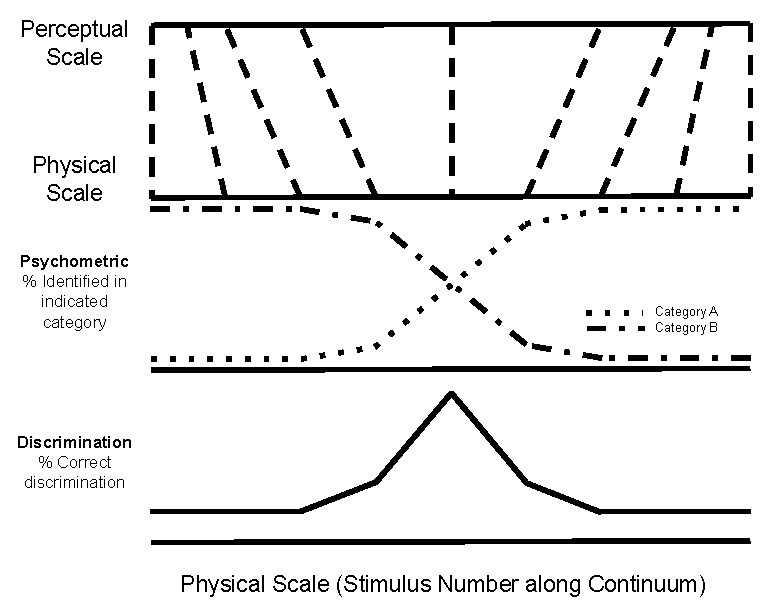
\includegraphics[width=0.75\textwidth]{figures/CP_def.pdf}
  \caption[A schematic of idealized categorical perception]
{A schematic of idealized categorical perception. \emph{Top}: The lower scale depicts a series of stimuli that are spaced a fixed distance apart according to some physical measure. In a perceptual representation of these stimuli the distances between adjacent stimuli may be modified in a way that groups the stimuli into categories as shown in the upper scale. \emph{Middle:} Idealized psychometric function or identification functions to illustrated the categorical perception of the nine stimuli distributed at equal intervals along the physical continuum. This is the percent identified in the indicated category plotted against the the stimulus number along the continuum, i.e. the physical scale. \emph{Bottom:} Discrimination function representing the increased sensitivity to changes in the stimuli near the categorical boundary.\index{cp}}
  \label{fig:cpdef}
\end{figure}

\subsection{Why European Starlings?}

European starlings ({\it Sturnus vulgaris}) are an excellent established model organism to study auditory processing and  categorical perception. Like human speech, starling song is composed of learned, spectrally complex, temporally-patterned acoustic objects (called \textit{\textbf{motifs}}), that are produced in long, well-organized temporal sequences \cite{gentner2003neuronal}, and that function in a wide range of natural behaviors. As with other complex natural signals, our understanding of how birdsongs are represented in higher cortical regions, both benefits from and is hindered by the complex spectro-temporal character of these sounds. Multiple physiological studies have used conspecific vocalizations, and reveal a strong selectivity for songs that emerges across the auditory forebrain and strengthens from field L to \ac{NCM} and \ac{CM} \cite{gentner2003neuronal, gentner2004neural, thompson2010song, jeanne2011emergence}.

European starlings (\textit{Sturnus vulgaris}) are an excellent established model organism to study auditory processing. Like human speech, a starling's song is composed of learned, complex temporally-patterned acoustic objects, called motifs, produced as part of a longer, well-organized temporal sequence\cite{gentner2003neuronal}. Starlings rely on object-level representations of motifs \cite{Meliza2010,p03702,Comins2013,comins2014auditory}, and the neural correlates of motif perception are localized in the regions of the auditory forebrain \emph{that are evolutionarily homologous to the mammalian auditory cortex\cite{wang2010laminar}}. 

The songbird auditory system follows the vertebrate plan\cite{Carr1992}. Field L2a is the primary telencephalic target of the auditory thalamus\cite{p05432}, and is the input layer for a columnar circuit spanning L1, L3, and \ac{CM}, anatomically\cite{Wang2010a,p10330}, genetically\cite{Dugas-Ford2012}, and functionally\cite{Calabrese2015} analogous to the mammalian auditory cortical micro-circuit. Field L sub-regions also project to the \ac{NCM}, a region that, a region that, along with the \ac{CLM}, shares reciprocal connections with the \ac{CMM}. Neurons in \ac{NCM} have been shown to have complex composite receptive fields\cite{kozlov2016central} that are reminiscent of the multidimensional receptive fields found in cat A1\cite{atencio2008cooperative}. Multidimensional receptive field characteristics can be reproduced by a \ac{DNN}\cite{kozlov2016central} trained to represent starling songs. Neurons throughout the avian cortex are selective for species-specific (conspecific) vocalizations\cite{Bonke1979,Leppelsack1976,Muller1985}, with selectivity increasing from Field L2, to L1 and L3\cite{Theunissen2004,Theunissen1998,Theunissen2000}, and again in \ac{NCM} and \ac{CM}\cite{Calabrese2015,Muller1985,Grace2003,Bonke1979,Leppelsack1976,p02120,Gentner2004,Thompson2010,Jeanne2011}. This is consistent with a functional hierarchy tuned to conspecific song\cite{Hsu2004,Woolley2005}, refined by experience\cite{p02120,Sockman2002,Sockman2005,Phan2006,Thompson2010,Jeanne2011}, with selectivity for acoustic features at multiple timescales increasing in a feed-forward manner\cite{Rose1988,Kaas2000,Binder2000,VanEssen1992}. Because of its compact organization, close relation to well-studied sensorimotor/vocal production structures, and the rich behavioral history of birdsong, the system is ideal for understanding the processing of natural acoustic communication signals.
Starlings respond to natural complex stimuli patterns such as the presence or absence of a center-embedded recursive structure\cite{gentner2006recursive,comins2014auditory,comins2014temporal}, a characteristic previously thought unique to human language (at least by Chomsky), allowing access to signals that would be invasive in humans, and cost prohibitive in non-human primates.

\subsection{The difficulties of using European Starlings}

However, the lack of parametric control over the complex acoustic features composing birdsongs (and other communication signals in other species) had rendered it difficult to more rigorously and extensively characterize both the information that these regions encode, and how this information is encoded. \comment{Do I need to put different straw-man theories here?} Ideally, we would like to parametrically control the complex natural stimuli to which high-order sensory regions are tuned, with the same precision and control that past studies have manipulated more simple stimuli like white noise and simple sine stimuli that can drive more primary sensory regions.

Genetic and viral tools

off the shelf hardware and solutions

increased mobility during chronic recordings (although michael long did get his headfixed 2 photon recording)

\subsection{What is required for \CP research?}

The fundamental difficulty with \CP research is that it generally occurs in the perception of a high dimensional space where naturally occurring ecologically relevant stimuli exist only on non-uniformly distributed sub-manifold of that space. In terms of auditory \CP in human speech, the high dimensional space is the space of all possible sounds that could possibly be heard, most of which would sound like random noise. The naturally occurring ecologically relevant stimuli is all the possible spoken sounds or phonemes that are useful for human speech production and comprehension, which exist in a much smaller lower-dimensional subset of all possible sounds. Even within this subset of sounds, not all possible phonemes are heard with equal probability and this distributional information may begin to shape our perceptual systems even before birth.

Because of this, the majority of auditory \CP has focused on human speech sounds, predominantly English, leveraging our intuitions and years of linguistic modelling to identify the relevant dimensions where \CP occur. \CP work concerning animal vocalizations must first identify stimuli that are categorically perceived, a process that was very labor intensive\cite{swamp sparrow series of papers} before the development of more modern techniques\cite{Tim's paper on distribution}. The variation within the songs of European starlings also make this easier because it is much easier to find song elements that are of distinct types.

Furthermore, the identification of category boundaries is more difficult in non-human research than with human subjects. Since we can't provide instructions, we are forced to use multiple shaping or pre-training stages of operant behavioral conditioning. Also, if we permit a fully adaptive double staircase procedure, our subjects learn to exploit this and force the boundary all the way to one side or another. To solve this we use a new staircase technique.

Last, but certainly not least, \CP requires the generation of a synthetic continuum between the categories or category exemplars. In human speech, the existence of speech synthesizers has made this task easy, at least in English. In Chinese for example, the technical difficulty in creating a Chinese-based synthetic continuum suitable for a \CP study has been proposed as a reason for the large number of papers focused on \CP in lexical tones in the Chinese language\cite{zhang2013categorical}. \CP research on animal vocalization has been limited to exploiting natural variation in recorded calls\cite{swamp sparrow cp} which invariably limits the sampling and control over the stimuli. It has also been shown that the quality of the speech synthesizer is correlated with how much \CP is observed\cite{something}.

Thus the approach we present streamlines the following steps for \CP research in non-human vocalizations:
\begin{enumerate}
    \item Identification of relevant dimensions where \CP occurs
    \item Identification of categorical boundaries
    \item Generation of a synthetic continuum between the categories/ category exemplars.
\end{enumerate}

\subsection{History of Categorical Perception}

There is a long history of categorical perception research.

The invention of the formant speech synthesizer known as the Pattern Playback at Haskins Laboratories\cite{patternplayback} made the discovery of \CP possible.
The Pattern Playback was a machine that converted pictures of the acoustic patterns of speech in the form of a spectrograms into sound using light.

\CP was initally described as the absolute definition of completely quantal perception where subjects would be unable to discriminate differences to stimuli within a category, only noticing differences in stimuli that lies across category boundaries\cite{liberman1957discrimination, Studdert1970motor}. Although only ever described as an idealized case, this definition is far too restrictive and has been disproven many times, however, it has caused much criticism of the work done in the \CP field with critics calling for ``The end of categorical perception as we know it''\cite{schouten2003end} etc.

Later work has instead demonstrated that with-category differences are discriminable\cite{pisoni1974reaction,carney1977noncategorical,massaro1983categorical} and meaningful\cite{miller1997internal,mcmurray2002gradient,mcmurray2008gradient}. Thus it seems there is just an increase in sensitivity to differences in stimuli that lie across category boundaries.

\CP first explored in 1957 concerning the discrimination of speech sounds within and across phenome boundaries\cite{liberman1957discrimination}.  In addition to dubbing the term ``Categorical Perception,'' Liberman suggested that \CP was unique to human speech, and furthermore, was what made human speech special. He also originally proposed the motor theory of speech perception\cite{liberman1967perception}.

Formerly thought to be peculiar to speech and color perception, \CP turns out to be far more general and may be a result of the way our neural circuits are wired to identify hierarchical patterns.

\CP also provides an intermediate explanation of equivalence classes which in turn form the basis of high-level symbolic thought.
Auditory \CP also forms the basis for human language

Previously thought auditory \CP to be strictly human trait possibly depending on special processing or that there might be some sort of motor theory basis that could inform perception based on a motor production model.
Now thought to be a ubiquitous feature of all perceptual systems.

It has been shown in chinchilla\cite{kuhl1975speech} and later in macaques\cite{kuhl1983enhanced}, that animal models also have enhanced discriminability at human phonetic boundaries without a phylogenetic history of phenomic knowledge, either acoustic or articulatory.
These studies consists of playing human speech sounds to animals and behaviorally measuring if they place the same boundaries we do.
This has been used to argue that human languages may have adapted to use phenome category boundaries located in regions with intrinsically higher discriminability\cite{stevens1981constraints,goldstone2010categorical}

There also exists a host of research on \CP in non-human vocal communication sounds. These studies either use
natural variation in the vocalizations
artificially generated hand drawn spectrogram morphs.
These studies are only possible after considerable background work establishes the relevant categories, similar to the techniques originally used in humans to identify \CP.

Categorical boundary location preference has also been explored, mostly in the context of human speech. Early explanations included the motor theory of speech perception which suggested that the explanation for \CP lay in the anatomy of speech production, specifically, physical differences during articulation\cite{liberman1967perception}. There have also been arguments made that a biological predisoposition influenced the development of human languages pushing phenome boundaries to locations of increased sensitivity\cite{stevens1981constraints, goldstone2010categorical, halle1979some}

\subsection{Learned Categorical Perception}

However, we also know that the boundary location is experience dependent. Native language exposure can shift boundary locations. Also, a sound difference that crosses a boundary of a language will be more discriminable to speakers of that language than to speakers of a language that doesn’t have a boundary in that location.

Lots more here about learning on \CP, also context dependency

\subsection{Our Contribution}
We use machine learning techniques to approximate unsupervised statistical learning of the distribution of the set of natural motifs while compressing it into a lower dimensional representation. This allows us to generate a continuum of synthetic motifs that lie between exemplars.

These types of machine learning methods allow for the creation of synthetic continua between exemplars when trained upon a corpus of that stimuli type. This allows for the exploration of natural ecologically relevant animal communication signals as we have done here. It also would allow the exploration of categorical perception in non-english languages. For example, technical difficulty in creating the Chinese-based synthetic continuum suitable for a \CP study has been proposed as a reason for the large number of papers focused on \CP in lexical tones in the Chinese language\cite{zhang2013categorical}.

Furthermore, stimulus naturalness has been shown to be a factor determining the degree of categorical perception, so as these machine learning techniques improve, we may be able to better explore the \CP phenomena.

This method allows for the creation or discovery of boundaries of \CP in an unsupervised way in animal vocalizations and are thus more ecologically relevant and will activate auditory regions that are specifically tuned to conspecific vocalizations.

\section{Results}
\subsubsection{Generating smoothly varying morphs}

\comment{
    Question / We need to show: parameterize complex natural stimuli\\
    Data / That is how we show: compressive generative deep learning\\
    Answer / We thus know: Able to generate smoothly varying morphs
    
    more on utility of method, demonstration
    descriptive demo of technique
    
    spend more time describing data, description of how much data is there

 motifs (song segments) of starling song. The DBN accomplishes a non-linear dimensionality reduction of the starling motif corpus to a low dimensional latent space (64 dimensions), as well as providing a generative model from any point in this latent space to a starling song-like sound. The trained DBN allows one to interpolate between any two arbitrarily chosen starling motifs projected into the latent space, to create a smoothly varying continuum of morphed motifs that shift from one target motif to the other, without sounding like a simple linear crossfade between them.
}

Using a large corpus of recorded starling song, a generative machine learning model is trained to non-linearly autoencode 400 mS motifs (song segments) of starling song in a low (64) dimensional latent space. The generative model attempts to model the distribution of song segments the model is trained on and as a result it tries to completely fill the latent space with projected representations (information bottleneck). The consequence of this is that for any point in the latent space, the spectrogram reconstruction of that point could lie within the actual distribution of starling song. Thus, the model can be used to interpolate between any two arbitrarily chosen starling motifs projected into the latent space to produce a smoothly varying continuum of morphed motifs that shift from one target motif to the other. Instead of sounding like a simple linear crossfade between the two motifs, the network tries to produce a motif that could be in the distribution of recorded motifs, resulting in more realistic sounding motifs.

\subsubsection{Behavioral Measurement of Perceptual Space}

\comment{
    Question / We need to show: Categorical behavioral responses on multiple dimensions\\
    Data / That is how we show: behavioral task, 4pl fits\\
    Answer / We thus know: Starlings will behaviorally respond to morphs between templates in a manner well described by a 4 parameter logistic curve
}

Starlings are trained on a two alternative choice task where four arbitrarily chosen motifs (labeled A, B, C, and D) are associated with a left response and another four (E, F, G, and H), are associated with a right response as summarized in figure \ref{fig:task-diagram}. After training to a stable performance criterion, the interpolated morph motifs generated by the \ac{DBN} are used to probe the bird's perception as each left-associated motif is transformed into each right-associated motif. We employed a ratcheting double staircase that \emph{allowed us to iteratively (and independently) estimate the categorical boundary along each of the 16 morph dimensions for each subject}. 

This provides independent binary behavioral responses along each of the 16 possible dimensions interpolating from each of the 4 left associated motifs to each of the right associated motifs. A \textit{\textbf{psychometric curve}} (four parameter logistic function) is fit to these behavioral responses and supplemental figure \ref{fig:something} demonstrates how well a four parameter psychometric curve fits the average response along a single example dimension. We measure 16 of these curves for each bird.

In all cases, birds show very clear categorical perception as evidenced by the steepness each psychometric function regardless of subject or motif dimension. Comparing the psychometric curves within a single bird across all 16 motif-to-motif dimensions reveals a large amount of variation in the point of subjective equality (the category boundary) and in how sensitive the bird is to stimulus changes across the boundary (Fig. \ref{fig:psychom-all}). This variability across dimensions is presumably a result of the non-linear nature of the \ac{DBN} song compression and morphing. Thus, we can conclude that \emph{the features the DBN uses to represent the motifs are perceptually relevant to the starlings}, and that the starlings are differentially sensitive to variation along these different feature dimensions.

Despite the significant variability within a single bird across multiple morph dimensions, we observed a remarkable degree of consensus between birds.  This included strong agreement in where each bird placed the category boundary on a given dimension, and in the sensitivity of all birds to changes along a given stimulus dimension (slope of psychometric function). Figure \ref{fig:share-psycho} gives an example of the typical agreement between subjects, where two of the 16 morph dimensions are plotted for 4 different birds.

Psychometric curves for four starlings, over several months of training, are highly conserved between individuals, suggesting a shared perceptual space. The y-axis shows the probability of a right response to a stimulus morphed continuously between, for example on the left, motif B (reinforced as left) and motif F (reinforced as right). The x-axis is the morph position between the left associated motif to the right associated motif.

\comment{
    Question / We need to show: independent between birds?\\
    Data / That is how we show: Boundary position and sensitivity are closer within a given dimension (offset biases are closer within a given subject)\\
    Answer / We thus know: Therefore they have a shared perceptual space
}

The left and right scaling parameters are statistically more conserved across all morphs within a single bird indicating that they are bird specific parameters as demonstrated by figure \ref{fig:???} and table \ref{tbl:???}. This makes sense because they correspond to the bird's absolute performance on the left and right endpoints. Figure \ref{fig:???} and table \ref{tbl:???} also show that the category boundary and the sensitivity are conserved within a given morph dimension across different subjects indicating a shared perceptual space of these synthetic natural-like sounds in these wild caught birds. 

\comment{
    Question / We need to show: not strictly stimulus/stim dims independent\\
    Data / That is how we show: birds trained on different categorical targets have predictably shifted boundaries\\
    Answer / We thus know: These dimensions are not all independent
}

The shared perceptual space for motif categorization may result from either common training and experience, idiosyncrasies of the compressive network transformation, or some combination of the two. To test for this, we permuted the initial motif category assignments for a subset of birds. Instead of associating motifs A, B, C and D with left responses and motifs E, F, G, and H with right responses, a new cohort of birds learned, for example, to associate motifs A, B, E, and F with left responses and motifs C, D, G, and H with right responses. Thus, a subset of the 16 interpolating morph dimensions between left and right associated motifs is shared with the original cohort's interpolating morph dimensions. Comparing these shared boundaries demonstrates that on some of the interpolated morph dimensions, both cohorts of birds place the boundaries in same location as shown in the left of figure \ref{fig:shift-psycho} while in other interpolating morph dimensions each cohort has a separate boundary (but consistent within that cohort), as shown in the right of figure \ref{fig:shift-psycho}. The boundaries that are preserved across motif category permutation indicate that these dimensions are independent from the other dimensions, however, the boundaries that are shifted as a result of the motif category permutation indicate an interaction between the interpolated morph dimensions. This is unexpected, especially if one considers that in the latent space of the DBN there is minimal collinearity and no discernable structure between any of the 8 motifs used.

\subsection{Artificial Neural Network Representation}

\comment{
    Question / We need to show: artificial neural population responses predict psychometric curves\\
    Data / That is how we show: hold one dimension out network predictions\\
    Answer / We thus know: how the animal responds in one sub-region of the parametrized space informs responses in other sub-regions
}

Another way to gauge the independence of the 16 interpolation dimensions is to use the representation learned by the DBN to predict the parameters of the behavioral psychometric function. Because we used the latent space to create linear, independent morphs, there isn't enough information on the relationships between the morph dimensions in the latent space alone to predict behavior. Using the activations of the entire DBN, however, can accurately predict (in a hold-one-out paradigm) the psychometric boundary and slope. Because this is a completely determined system with no noise we can show that the mean square error between the curve predicted by the logistic regression and the behaviorally determined psychometric curve is less than would be expected if the psychometric curves are randomly shuffled. Thus, the stimulus dimensions used for categorization are not independent of each other.  Knowing how the subjects respond in one sub-region of the latent space reveals information about how other portions of the space are perceived.

\subsubsection*{Electrophysiological Recordings}

\comment{
    Question / We need to show: recordings from secondary auditory regions with extremely timelocked responses\\
    Data / That is how we show: gaussian convolved psth\\
    Answer / We thus know: \\
    
    Question / We need to show: neural responses encode stimuli dimensions\\
    Data / That is how we show: \\
    Answer / We thus know: \\
    
    Question / We need to show: neural responses vary along morph dimension\\
    Data / That is how we show: \\
    Answer / We thus know: \\
    
    Question / We need to show: neural population responses predict psychometric curves\\
    Data / That is how we show: hold one dimension out neural predictions\\
    Answer / We thus know: secondary auditory regions encode boundary locations
    
    Question / We need to show: differences in neural rep, based on experience\\
    Data / That is how we show: comparisons of p values for different recording blocks\\
    Answer / We thus know: no difference in representations in terms of ability to predict boundary parameters
    
    more of a methods summary, summary of number of recordings and neurons, err in more in results
}

To explore the neural underpinnings of categorical perception we record from secondary auditory regions of anesthetized starlings and present the generated motifs. We record from a total of 2019 neurons in <<<TODO>>> sites in 8 different starlings, 4 trained, 4 naive, never having heard the stimuli before. We use a 32 channel silicon electrode and stereotaxically target \ac{CMM} and \ac{CLM} as described in the methods and shown in figure \ref{}. We sort the data using MountainSort\cite{mountainsort}. 

We find the units are extremely time-locked and stimuli specific as demonstrated by figure \ref{}. Because of this we choose to include time in our neural representation by convolving the spike train with a Gaussian($\sigma = \SI{10}{ms}$). This provides us with a continuous estimate of firing rate through time for each trial for every unit. If we look at the average of this representation as we move along a morph dimension we find that there is a large amount of variation in how the units respond. Some units respond very smoothly to changes along a morph dimension, whereas others are quite categorical.

We restrict our analysis to units that are able to correctly identify the identity of our eight template motifs (averaged in a pairwise fashion so that 50\% is chance) more than 60\% of the time. This leaves 705 remaining "good" units as seen in figure \ref{}.

Using the hold-one-dimension-out prediction strategy, similar to that for the DBN activations, we predicted the behavioral psychometric functions from the neural population representations. The behavioral response is fit given the neural representation of stimuli presented from 15 of the 16 interpolated morph dimensions and then the response is predicted on the neural responses of the remaining dimension. For computational tractability we reduced the dimensionality of the neural representation to 24 dimensions using an LDA-like method. The mean squared error for each held out dimension are combined to provide 16 performances for each neural recording (39?) for each set of behaviorally determined psychometric fits (8). Once again we create a null distribution by shuffling the labels of the morph dimensions 2048 times and measuring the KS distance to distribution of 16 dimension performances. Overall we find the fits are significantly better than would we expected by chance. Furthermore, if we compare the distribution of p values for recordings from untrained naive birds against the recordings of the birds that had been behaviorally trained we find that there's no difference between how well the neural representation of naive birds or trained birds can predict the location of the boundary or the sensitivity to changes near the boundary. That is not to say that there is no difference between the population representation in trained or untrained birds, or that more information about boundary location isn't encoded elsewhere in the brain, but that the information that allows generalization of categorical boundary parameters to other morph dimensions is equally present in both trained and untrained birds.

\comment{
Change this to UMAP of end clusters,
show a single dimension
before neurometric stuff/logistic stuff

Visualizing the neural population representation (concatenating all the individual unit representations) of the presentations of the 8 original template motifs using tSNE reveals a high degree of separation between clusters of different stimuli as seen in figure \ref{fig:tsne}. Similar patterns are observed in naive and trained animals, regardless of whether they've heard the stimuli before the neural recording. 
}

/subsection{The Thielk Curve}

We are interested in the brain's ability to discriminate changes along our morph dimension. We use distance in our neural representation to approximate the brain's ability to discriminate. 

We pose the following regression problem by defining the Thielk curve
$T(x): x \in [1, 128]$, such that for a pair of presented stimuli, $a$ and $b$, and a distance, $y$ in neural representation space between these to presentations, $y = \int_a^bC(x)dx + \epsilon$ for $a,b \in \{p_1, p_2, ... p_n\}$ for some small $n$ and $p_i \in [1, 128]$. This assumes that the neural representation of these stimuli smoothly vary (up to some noise) as I move along the morph dimension. We then perform the regression to minimize the \MSE of $\epsilon$ for all pairs of stimuli presented on a single morph dimension.

We would like the Thielk curve $T(x)$ to have the following properties: 1. Strictly positive. 2. Smooth over the range $[1, 128]$.
To keep the function positive I have used $C(x)=e^{f(x)}$ and to keep it smooth I have used $f(x)$ as a polynomial

\section{Discussion}
\comment{
  Results -> Conclusion\\
    We found: Existence of shared perceptual space, that measurable features that could be extrapolated from representations of a machine learning model trained to represent starling song, as well as neural\\ activity of tens of neurons in the secondary auditory regions of starlings.\\
    We filled gap: Generative Machine learning techniques allow exploration of complex natural stimuli and therefore the responses of secondary perceptual regions. naturally occurring categorical perception
}

Our results overcome a long-standing impediment to understanding the perception of natural communication signals. We demonstrate a method for parametrizing complex stimuli and generating \emph{smoothly varying morphs between these stimuli}, as well as how to use these morphs to explore the perceptual basis, behaviorally and neurally, of the natural stimulus space. To our knowledge, this marks one of the first naturalistic parametric explorations of non-human auditory communication signals. Our characterization of the perception of this space and its neurological underpinnings, reveals remarkable behavioral consensus between animals for categorical boundaries and a broadly distributed encoding strategy for categorical stimulus information at the neural population level.  

The work demonstrates the existence of a shared perceptual space, common across individuals, in which perceived categorical boundaries cluster at consensus locations.  This kind of consensus is a pre-requisite to functional communication systems that use discrete signals.  Furthermore, the 16 interpolating morph dimensions used in this study are not independent, nor are they a simple linear function of the endpoints, independent of the structure of the network space. If the latter were true, then all (or none) of the boundaries would shift when the endpoints were permuted. Instead, because only some of the dimensions are affected by permutation of the initial categories, not all the dimensions are independent, and the relationships between them are likely complex. Moreover, because there are dimensions that are not changed by the permutation of the initial categories, the decision boundaries learned by birds cannot rely on simple separation of the initial template motifs (as are seen in algorithms such as support vector machines or equivalent). Understanding where these boundaries fall likely requires knowledge of how natural stimuli is distributed in the latent space of the network, and the underlying geometry in which the latent manifold is embedded. Additional work is needed in these areas. \cite{tims paper}

\comment{
  Limitations in filling gap\\
    Our limitation: better generative machine learning model\\
    Details: ml is a rapidly changing field\\
    How to interpret / fix: GAIA
}

The field of machine learning is rapidly evolving and there are number of possible improvements to the processing and methodology, however, this work mainly demonstrates the usefulness of these kinds of techniques for understanding the perception of complex natural communication signals. In addition to changes in network architecture, newer implementations of spectrogram inversion would improve stimulus generation and are currently being tested and developed. In our experiment, however, different initializations of the spectrogram inversion process revealed that neurons in \ac{CM} are sensitive to these small physical differences in physical stimuli that are imperceptible to human ears figure \ref{fig:tsne}.

\comment{
  Limitations in generalization
    Our limitation: limited stimuli set\\
    Details: we approximate natural experience with dataset\\
    How to interpret / fix: changing distribution of experienced song before training influence category boundary?
}

The network representation decoding of the psychophysical parameters indicates the importance of the distribution of natural songs on the perceptual space. While our library of songs provides for an approximation of their natural experience history, it is limited, especially in the context of wild caught animals. A fascinating future direction of this work would be to see if changing the distribution of experienced song before the training would influence category boundaries.

Our ability to predict held out behavioral responses from both the artificial neural network activations as well as the in vivo neural population activities indicate that each of these representations are sufficient, although not uniquely so, to describe the perceptual and behavioral space. One compelling result is that the behavior generalizes across this stimulus space, such that that knowing how perception acts in one sub-region can inform behavioral responses in other sub-regions. This category generalization also deserves further study.

Finally, the fact that categorical behavioral responses can be decoded from a randomly selected set of 10s of neurons contributes to a growing body of work \cite{jeanne2011emergence,kozlov2016central} that opposes the strongest version of sparse hierarchical models of perception, where neurons with simpler receptive fields converge onto neurons with a more complex receptive fields until a complex percept, like Jennifer Aniston emerges \cite{quiroga2005invariant}. Under this model, decoding a categorical behavioral measure (as we show here) is only possible by matching the right stimuli to the right subset of neurons. Thus, our results imply that \emph{the representation of these secondary auditory regions is much more distributed than would be predicted by a model where increasingly complex features are encoded exclusively by single neurons}.

Using A DBN as a generative model of birdsong is another limitation of this work due to the amount of recent progress in machine learning. In particular, we recommend using \cite{GAIA} for these techniques as it can produce much more realistic sounding birdsong and is explicitly constructed such that the stimuli space is convex and interpolations between exemplars are realistic.

\comment{
  Limits in generalization\\
    Our limitation: anesthetized\\
    Details: different network state?\\
    How to interpret / fix: might not measure actual awake representations or effects of attention but certainly measuring network tendencies. long term awake chronic recording
}

Another possible limitation of these results is the anesthetized recording prep that was used. These measurements might not necessarily reflect the actual awake representations, and especially attentional modulation but certainly measure the functional tendencies of the network representation. Additionally, this doesn't change our interpretation which is based on the fact that we can predict categorical boundary parameters and not precisely what representation we are using to make the prediction.

\comment{
  Limits in generalization\\
    Our limitation: avian\\
    Details: homologous, but structural differences\\
    How to interpret / fix: only other species that recognizes complex hierarchical features and recursive grammars is humans, but this line of work can perhaps indicate what kinds of patterns to look for in a system that has solved similar problems. Approach can also be used for vision.
}

While regions of the auditory forebrain are homologous to mammalian auditory cortex\cite{wang2010laminar}, there are significant structural differences. Thus, while solutions to categorical perception of complex auditory stimuli used by birds aren't necessarily the same as those in our own, they do ...  

\comment{
  Limits in generalization\\
    Our limitation: causal\\
    Details: ability to decode perceptual measurements, doesn't necessarily mean that the bird is using it.\\
    How to interpret / fix: opto/viral, not as many tools in wild caught animals. Same kind of efficiency arguments, indicates where to look.

  Contributions beyond / Science is better now\\
    Our strength: solved long standing impediment to working with complex natural stimuli\\
    What it is useful for: higher order perceptual neuro, categorical \\
    The difference made: defeat the curse of dimensionality that has plagued...
}